% 20190312
% 20191108

\frenchspacing

\begin{frame}[fragile]{标记语言:另一种排版方式}
	电子文档软件\footnote{如 Microsoft Word}用鼠标或快捷键选择字体形状\par
	标记语言利用\uline{纯文本标记}指示字体形状,更容易控制\par
	\begin{igsimple}
		Some \textit{italicized} words
		\begin{itemize}\leftskip=-4em
			\item HTML:\txt{Some \uline{<i>}italicized\uline{</i>} words}
			\item Markdown:\txt{Some \uline{*}italicized\uline{*} words}
			\item \TeX{}:\txt{Some \uline{\{\string\itshape\ }italicized\uline{\string\/\}} words}
			\item \LaTeX{}:\txt{Some \uline{\string\textit\{}italicized\uline{\}} words}
		\end{itemize}\par
	\end{igsimple}\par
	学名 \textit{Allium hookeri} var. \textit{muliense} Airy Shaw 用 Markdown 表示\\
	\hfill\txt{\uline{*}Allium hookeri\uline{*} var. \uline{*}muliense\uline{*} Airy Shaw}\hfill\hbox{}\par
	字体形状由位置决定,可以由确定的规则描述,故可以自动化
\end{frame}

\begin{frame}[fragile]{利用正则表达式控制字体形状}
	\catcode`\×=13
	\def×{\makebox[1em][c]{$\times$}}
	\centering
	\begin{minipage}[c]{61.5ex}
		\begin{YVerb}[showspaces=false,codes={\catcode`\×=13}]
			Allium fistulosum L.
			Allium caput-medusae Airy Shaw
			Allium hookeri var. muliense Airy Shaw
			Allium senescens subsp. glaucum (Regel) Dostál
			Allium ×proliferum (Moench) Schrad. ex Willd.
			Allium giganteum 'Ambassador'
			Allium 'Gladiator'
		\end{YVerb}
	\end{minipage}
	\par
	\hbox{}\hfill
	\begin{minipage}[c]{57.5ex}
		\begin{enumerate}
			\item<0> !^(\u\l+) ([\l-]+) ! \replace ! \*\1 \2\* !
			\item<0> !(?<= var\. )([\l-]+) ! \replace ! \*\1\* !
			\item<0> !(?<= subsp\. )([\l-]+) ! \replace ! \*\1\* !
			\item<0> !^(\u\l+) ! \replace ! \*\1\* !
			\item<0> !(?<=×)([\l-]+) ! \replace ! \*\1\* !
		\end{enumerate}
	\end{minipage}\hfill\par
\end{frame}

\printbookmarkfalse
\begin{frame}[fragile]{利用正则表达式控制字体形状}
	\catcode`\×=13
	\def×{\makebox[1em][c]{$\times$}}
	\centering
	\begin{minipage}[c]{61.5ex}
		\begin{YVerb}[commandchars=\\\{\},showspaces=false,codes={\catcode`\×=13}]
			*Allium fistulosum* L.
			*Allium caput-medusae* Airy Shaw
			*Allium hookeri* var. muliense Airy Shaw
			*Allium senescens* subsp. glaucum (Regel) Dostál
			Allium ×proliferum (Moench) Schrad. ex Willd.
			*Allium giganteum* 'Ambassador'
			Allium 'Gladiator'
		\end{YVerb}
	\end{minipage}
	\par
	\hbox{}\hfill
	\begin{minipage}[c]{57.5ex}
		\begin{enumerate}
			\item<1> !^(\u\l+) ([\l-]+) ! \replace ! \*\1 \2\* !
			\item<0> !(?<= var\. )([\l-]+) ! \replace ! \*\1\* !
			\item<0> !(?<= subsp\. )([\l-]+) ! \replace ! \*\1\* !
			\item<0> !^(\u\l+) ! \replace ! \*\1\* !
			\item<0> !(?<=×)([\l-]+) ! \replace ! \*\1\* !
		\end{enumerate}
	\end{minipage}\hfill\par
\end{frame}

\begin{frame}[fragile]{利用正则表达式控制字体形状}
	\catcode`\×=13
	\def×{\makebox[1em][c]{$\times$}}
	\centering
	\begin{minipage}[c]{61.5ex}
		\begin{YVerb}[commandchars=\\\{\},showspaces=false,codes={\catcode`\×=13}]
			*Allium fistulosum* L.
			*Allium caput-medusae* Airy Shaw
			*Allium hookeri* var. *muliense* Airy Shaw
			*Allium senescens* subsp. glaucum (Regel) Dostál
			Allium ×proliferum (Moench) Schrad. ex Willd.
			*Allium giganteum* 'Ambassador'
			Allium 'Gladiator'
		\end{YVerb}
	\end{minipage}
	\par
	\hbox{}\hfill
	\begin{minipage}[c]{57.5ex}
		\begin{enumerate}
			\item<1> !^(\u\l+) ([\l-]+) ! \replace ! \*\1 \2\* !
			\item<1> !(?<= var\. )([\l-]+) ! \replace ! \*\1\* !
			\item<0> !(?<= subsp\. )([\l-]+) ! \replace ! \*\1\* !
			\item<0> !^(\u\l+) ! \replace ! \*\1\* !
			\item<0> !(?<=×)([\l-]+) ! \replace ! \*\1\* !
		\end{enumerate}
	\end{minipage}\hfill\par
\end{frame}

\begin{frame}[fragile]{利用正则表达式控制字体形状}
	\catcode`\×=13
	\def×{\makebox[1em][c]{$\times$}}
	\centering
	\begin{minipage}[c]{61.5ex}
		\begin{YVerb}[commandchars=\\\{\},showspaces=false,codes={\catcode`\×=13}]
			*Allium fistulosum* L.
			*Allium caput-medusae* Airy Shaw
			*Allium hookeri* var. *muliense* Airy Shaw
			*Allium senescens* subsp. *glaucum* (Regel) Dostál
			Allium ×proliferum (Moench) Schrad. ex Willd.
			*Allium giganteum* 'Ambassador'
			Allium 'Gladiator'
		\end{YVerb}
	\end{minipage}
	\par
	\hbox{}\hfill
	\begin{minipage}[c]{57.5ex}
		\begin{enumerate}
			\item<1> !^(\u\l+) ([\l-]+) ! \replace ! \*\1 \2\* !
			\item<1> !(?<= var\. )([\l-]+) ! \replace ! \*\1\* !
			\item<1> !(?<= subsp\. )([\l-]+) ! \replace ! \*\1\* !
			\item<0> !^(\u\l+) ! \replace ! \*\1\* !
			\item<0> !(?<=×)([\l-]+) ! \replace ! \*\1\* !
		\end{enumerate}
	\end{minipage}\hfill\par
\end{frame}

\begin{frame}[fragile]{利用正则表达式控制字体形状}
	\catcode`\×=13
	\def×{\makebox[1em][c]{$\times$}}
	\centering
	\begin{minipage}[c]{61.5ex}
		\begin{YVerb}[commandchars=\\\{\},showspaces=false,codes={\catcode`\×=13}]
			*Allium fistulosum* L.
			*Allium caput-medusae* Airy Shaw
			*Allium hookeri* var. *muliense* Airy Shaw
			*Allium senescens* subsp. *glaucum* (Regel) Dostál
			*Allium* ×proliferum (Moench) Schrad. ex Willd.
			*Allium giganteum* 'Ambassador'
			*Allium* 'Gladiator'
		\end{YVerb}
	\end{minipage}
	\par
	\hbox{}\hfill
	\begin{minipage}[c]{57.5ex}
		\begin{enumerate}
			\item<1> !^(\u\l+) ([\l-]+) ! \replace ! \*\1 \2\* !
			\item<1> !(?<= var\. )([\l-]+) ! \replace ! \*\1\* !
			\item<1> !(?<= subsp\. )([\l-]+) ! \replace ! \*\1\* !
			\item<1> !^(\u\l+) ! \replace ! \*\1\* !
			\item<0> !(?<=×)([\l-]+) ! \replace ! \*\1\* !
		\end{enumerate}
	\end{minipage}\hfill\par
\end{frame}

\begin{frame}[fragile]{利用正则表达式控制字体形状}
	\catcode`\×=13
	\def×{\makebox[1em][c]{$\times$}}
	\centering
	\begin{minipage}[c]{61.5ex}
		\begin{YVerb}[commandchars=\\\{\},showspaces=false,codes={\catcode`\×=13}]
			*Allium fistulosum* L.
			*Allium caput-medusae* Airy Shaw
			*Allium hookeri* var. *muliense* Airy Shaw
			*Allium senescens* subsp. *glaucum* (Regel) Dostál
			*Allium* ×*proliferum* (Moench) Schrad. ex Willd.
			*Allium giganteum* 'Ambassador'
			*Allium* 'Gladiator'
		\end{YVerb}
	\end{minipage}
	\par
	\hbox{}\hfill
	\begin{minipage}[c]{57.5ex}
		\begin{enumerate}
			\item<1> !^(\u\l+) ([\l-]+) ! \replace ! \*\1 \2\* !
			\item<1> !(?<= var\. )([\l-]+) ! \replace ! \*\1\* !
			\item<1> !(?<= subsp\. )([\l-]+) ! \replace ! \*\1\* !
			\item<1> !^(\u\l+) ! \replace ! \*\1\* !
			\item<1> !(?<=×)([\l-]+) ! \replace ! \*\1\* !
		\end{enumerate}
	\end{minipage}\hfill\par
\end{frame}

\printbookmarktrue
\begin{frame}{如何应用于电子文档?}
	\parindent=1em
	\begin{enumerate}
		\item 用 Markdown 解释器处理成带字体风格的文本
		\item 将带字体风格的文本粘贴到电子文档中
	\end{enumerate}\par
	在线 Markdown 解释器:\texttt{https://dillinger.io/}\par
	\parindent=0em
	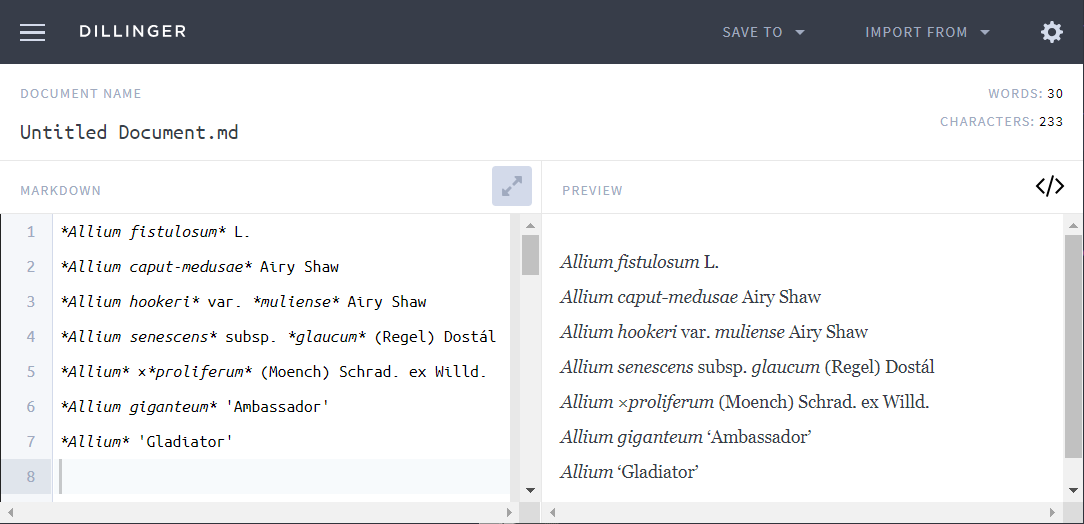
\includegraphics[width=\textwidth]{Illustratio/Markdown_online.png}
\end{frame}
